% \section{TCAN Model}

% % Reemplaza el frame "Problem Formulation" con este NUEVO frame combinado

% \begin{frame}{TCAN Model}
% \begin{columns}[T]
% \column{0.85\textwidth}
% \textbf{ \small Model Definition}
% \begin{itemize}
%     \item \scriptsize TCAN: Temporal Convolutional Attention Network.
%     \item \scriptsize Feed-forward autoregressive model (each prediction becomes input for the next step).
%     \item \scriptsize Controller in NFTM framework.
% \end{itemize}

% \textbf{\small Continuous Field}
% \begin{itemize}
%     \item \scriptsize $f_t$: snapshot of PDE solution.
%     \item \scriptsize Vector of size $N$ (spatial positions).
%     \item \scriptsize $f_t = [u(x_1,t), \ldots, u(x_N,t)]$.
%     \item \scriptsize Shape: $(1 \times N)$.
% \end{itemize}

% \textbf{\small Input and Output of the Model}\\
% \vspace{0.1cm}
% \scriptsize To predict $f_{t+1}$, the corresponding input and output of the model are:
% \begin{itemize}
%     \item \scriptsize \textbf{Input}: \textbf{history window} (chunk of $W$ previous fields): $[f_{t - W + 1}, f_{t - W + 2}, ..., f_{t}]$ with size $(B, W, N)$.
%     \item \scriptsize \textbf{Output}: \textbf{prediction of the field at next time step $t+1$}: $\hat{f}_{t+1}$, with size: $(B, 1, N)$.
% \end{itemize}

% \column{0.3\textwidth}
% \begin{tikzpicture}[scale=0.25]

% \node[rectangle, draw, fill=orange!20,
%       text width=1.4cm, align=center,
%       minimum height=0.65cm] 
% (input) at (0, 15.5) {\scriptsize History\\$(B,W,N)$};

% \node[rectangle, draw, fill=blue!20,
%       text width=1.4cm, align=center,
%       minimum height=0.65cm] 
% (tcan) at (0, 5.5) {\scriptsize TCAN\\Controller};

% \node[rectangle, draw, fill=green!20,
%       text width=1.4cm, align=center,
%       minimum height=0.65cm] 
% (output) at (0, -3.5) {\scriptsize Next Field\\$(B,1,N)$};

% \draw[->, thick] (input) -- (tcan);
% \draw[->, thick] (tcan) -- (output);
% \draw[->, thick, dashed, blue] (output.east)
%       to[bend right=30] node[right, font=\tiny] {rollout} (input.east);

% \end{tikzpicture}
% \end{columns}
% \end{frame}

% \begin{frame}
% \vspace{0.2cm}
% \small \textbf{Autoregressive Roll-out Process}\\
% \vspace{0.1cm}
% \begin{itemize}
%     \item \scriptsize Each TCAN call predicts next field from current window
%     \item \scriptsize Window slides: drop oldest, add prediction
%     \item \scriptsize Process repeats autoregressively for full trajectory
% \end{itemize}
% \scriptsize In the example below, the model first predicts $f_{21}$ from the window $[f_1,\dots,f_{20}]$, then uses the updated window $[f_2,\dots,f_{20},f_{21}]$ to predict $f_{22}$, and so on.
% \vspace{0.2cm}

% \begin{center}
% \resizebox{0.3\textwidth}{!}{%
% \begin{tikzpicture}[
%     box/.style={draw, rectangle, rounded corners, minimum width=2.2cm, minimum height=0.8cm, align=center, fill=orange!20, font=\small},
%     pred/.style={draw, rectangle, rounded corners, minimum width=1.6cm, minimum height=0.8cm, align=center, fill=green!20, font=\small},
%     arrow/.style={->, thick, >=stealth},
%     node distance=1.4cm
% ]

% % Step 1
% \node[box] (w1) {Window\\$[f_1,\dots,f_{20}]$};
% \node[pred, right=of w1] (p21) {$\hat{f}_{21}$};
% \node[font=\scriptsize, above=0.10cm of $(w1)!0.52!(p21)$] {TCAN};
% \draw[arrow] (w1.east) -- (p21.west);

% % Step 2
% \node[box, below=of w1] (w2) {Window\\$[f_2,\dots,f_{20},\hat{f}_{21}]$};
% \node[pred, right=of w2] (p22) {$\hat{f}_{22}$};
% \node[font=\scriptsize, above=-0.55cm of $(w2)!0.55!(p22)$] {TCAN};
% \draw[arrow] (w2.east) -- (p22.west);

% % Step 3
% \node[box, below=of w2] (w3) {Window\\$[f_3,\dots,f_{21},\hat{f}_{22}]$};
% \node[pred, right=of w3] (p23) {$\hat{f}_{23}$};
% \node[font=\scriptsize, above=-0.45cm of $(w3)!0.55!(p23)$] {TCAN};
% \draw[arrow] (w3.east) -- (p23.west);

% % Pred → next window (curvas por debajo, lejos del texto TCAN)
% \draw[arrow] (p21.south) to[out=-60,in=20] (w2.north);
% \draw[arrow] (p22.south) to[out=-60,in=20] (w3.north);

% % Continuation dots
% \node[font=\large] (dots) at ($(w3.south)!0.5!(p23.south) + (0,-1.2)$) {$\dots$};

% \end{tikzpicture}%
% }
% \end{center}
% \end{frame}

% \begin{frame}
% \small \textbf{TCAN Architecture}
% \begin{columns}[T]
%     \column{0.35\textwidth}
%     \begin{center}
%     \resizebox{1.25\textwidth}{!}{%
%     \begin{tikzpicture}[
%         box/.style={rectangle, draw, rounded corners, minimum width=2.4cm, minimum height=0.85cm, align=center, fill=blue!10},
%         op/.style={rectangle, draw, rounded corners, minimum width=2.4cm, minimum height=0.85cm, align=center, fill=green!10},
%         arrow/.style={->, thick, >=stealth},
%         input/.style={rectangle, draw, rounded corners, minimum width=2.4cm, minimum height=1.0cm, align=center, fill=orange!20},
%         output/.style={rectangle, draw, rounded corners, minimum width=2.4cm, minimum height=1.0cm, align=center, fill=red!20},
%         node distance=2.0cm and 1.6cm
%     ]
%     % Main flow - left column
%     \node[input] (input) {INPUT\\$f_{\text{history}}$};
%     \node[op, below=of input] (embed) {Embedding\\Conv1d+GELU};
%     \node[box, below=of embed] (features) {Features\\$(B,20,32,N)$};

%     % Attention column - center-right
%     \node[box, right=1.8cm of features] (query) {Query $Q$\\(last frame)};
%     \node[op, below=of query] (attn) {Causal\\Attention};
%     \node[box, below=of attn] (context) {Context\\$(B,32,N)$};

%     % Decoder/output column - right
%     \node[op, right=1.8cm of context] (decoder) {Decoder\\Conv1d};
%     \node[box, below=of decoder] (corr) {Correction\\$\tanh(\times0.1)$};
%     \node[output, below=of corr] (output) {OUTPUT \\$f_{\text{next}}$};

%     % CLEAN ARROWS - NO CROSSING
%     \draw[arrow] (input) -- (embed);
%     \draw[arrow] (embed) -- (features);
%     \draw[arrow] (features) -| ([xshift=-0.3cm]query.west) -- (query);
%     \draw[arrow] (query) -- (attn);
%     \draw[arrow] (attn) -- (context);
%     \draw[arrow] (context) -- (decoder);
%     \draw[arrow] (decoder) -- (corr);
%     \draw[arrow] (corr) -- (output);

%     % Residual from features to context (ABOVE)
%     \draw[arrow, dashed, blue] (features.south) 
%         to[out=-5,in=150] node[above, font=\footnotesize, black]{residual} 
%         (context.west);

%     % FIXED: LEFT→DOWN→RIGHT path from input to output
%     \draw[arrow, dashed, orange, thick] (input.south) 
%         |- ++(-2,0)     % LEFT (west)
%         |- ++(0,-18)     % DOWN (south) 
%         -| (output.west)     % RIGHT to output
%         node[below, font=\scriptsize, pos=0.1]{$f_t$};


%     % KV note
%     \node[font=\footnotesize, align=center, right=0.2cm of query, anchor=west] (kv) {$K,V$\\all frames};
%     \end{tikzpicture}%
%     }
%     \end{center}
    
%     \column{0.6\textwidth}
%     \begin{itemize}
%       \item \scriptsize \textbf{$f_{\text{history}}$}: chunk of 20 previous fields, size: $(B,20,N)$.
%       \item \scriptsize \textbf{Conv1d+GELU}: maps each field into its embedding of 32 features ($1\to32$ channels).
%       \item \scriptsize \textbf{Features}: reorganizes embeddings into temporal sequences, new tensor shape: $(B,20,32,N)$.
%       \item \scriptsize \textbf{Query $Q$}: extracts features from the most recent field $f_{t}$ and applies $1 \times 1$ convolution to generate query vectors.
%       \item \scriptsize $\mathbf{K},\mathbf{V}$: projects all $W$ embedded fields through separate $1 \times 1$ convolutions to produce keys $K$ and values $V$. 
%       \item \scriptsize \textbf{Causal Attention}: computes causal attention scores for each spatial position n: $\alpha_{w,n}=\text{softmax}_w(QK^T/\sqrt{32})$.
%       \item \scriptsize \textbf{Decoder}: translates temporal attention context into the spatial update: $\Delta f$.
%       \item \scriptsize \textbf{$f_{\text{next}}$}: $f_t+\Delta f$.
%     \end{itemize}
%   \end{columns}
% \end{frame}

% \begin{frame}
%   \small \textbf{Results with TCAN Controller}\\
%     \vspace{0.6cm}
%     \centering
%     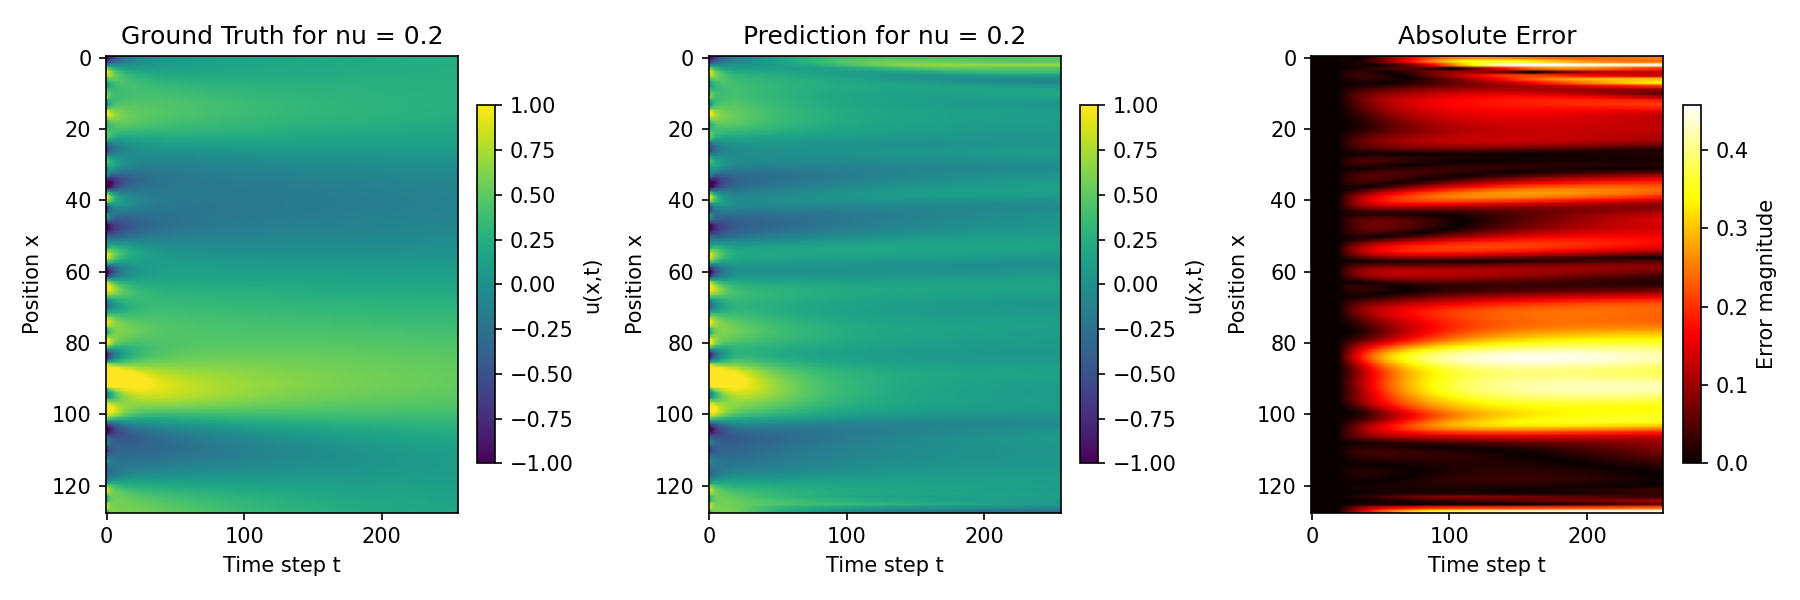
\includegraphics[width=0.55\textwidth]{images/TCAN/trajectory_epoch_0_nu0.2.png}
%     {\tiny Epoch 0}

%     \vspace{0.3cm}
%     \centering
%     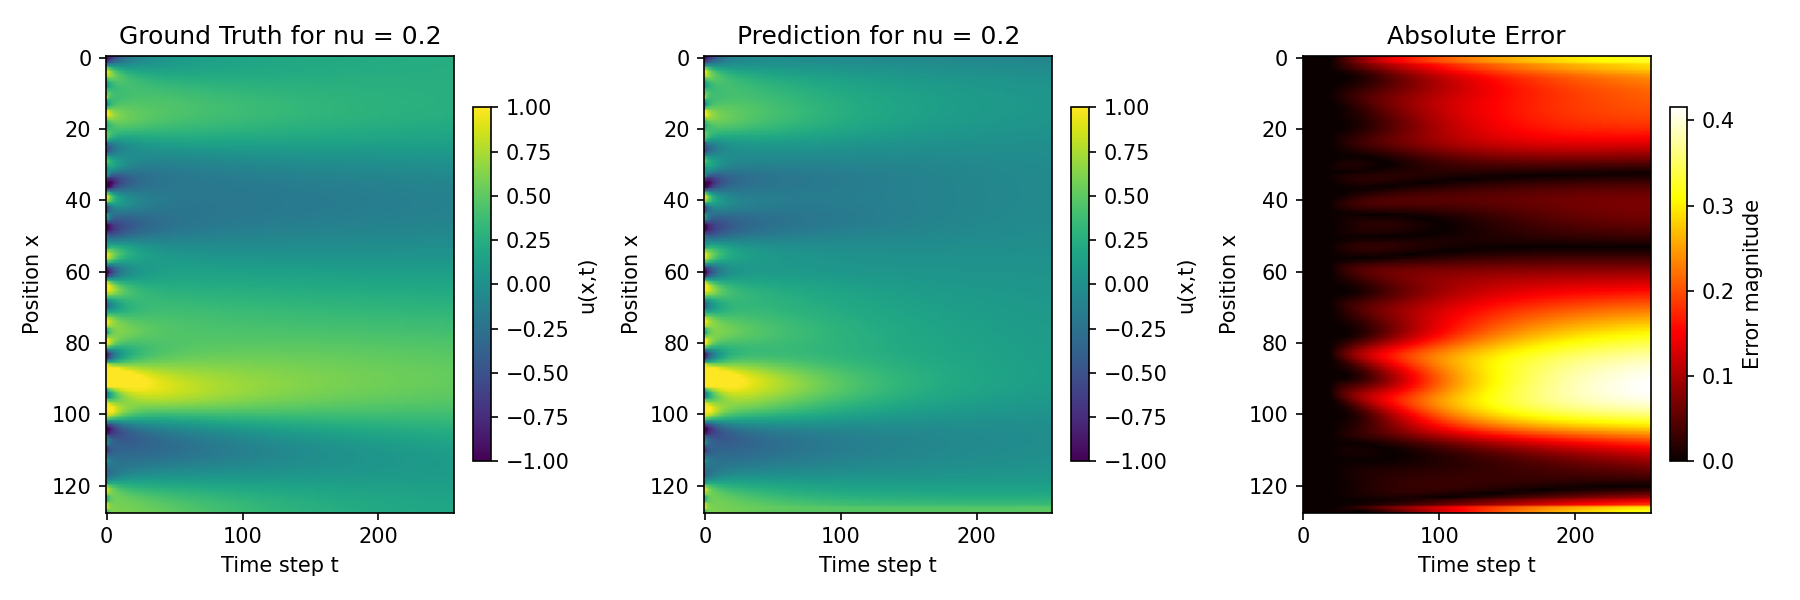
\includegraphics[width=0.55\textwidth]{images/TCAN/trajectory_epoch_40_nu0.2.png}
%     {\tiny Epoch 40}
  
%   \vspace{0.3cm}
%   \centering
%   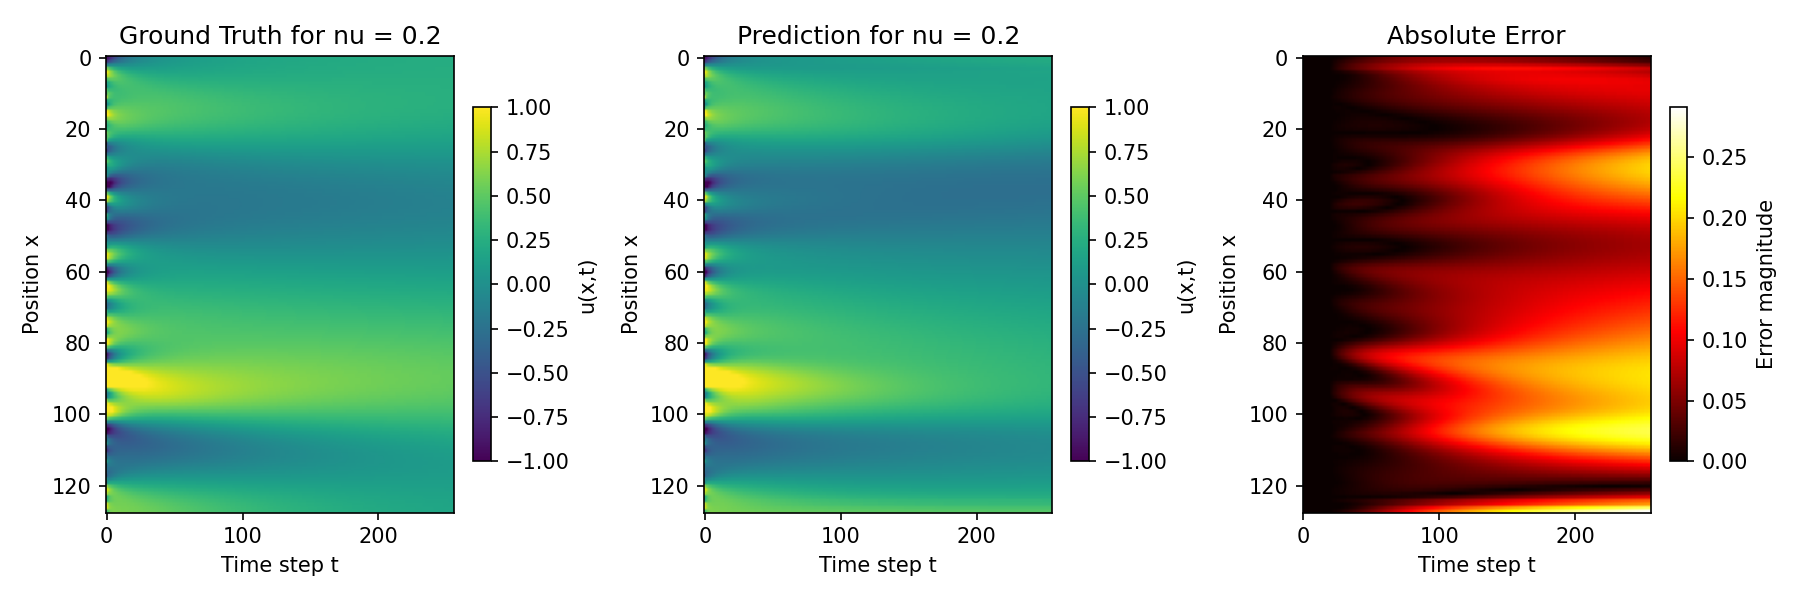
\includegraphics[width=0.55\textwidth]{images/TCAN/trajectory_epoch_80_nu0.2.png}
%   {\tiny Epoch 80}
% \end{frame}

\section{TCAN Model}

\begin{frame}{Why TCAN? Model Selection}

  \begin{block}{Three candidate architectures evaluated}
    \begin{center}
    \small
    \begin{tabular}{lccc}
      \toprule
      Architecture & Rel.\ $L^2$ ($s$=256) & Stable rollout & Resolution-robust \\
      \midrule
      CNN (ConvNet)    & 0.062 & short  & $\times$ \\
      Transformer      & 0.031 & medium & \checkmark \\
      \textbf{TCAN}   & \textbf{0.019} & \textbf{long} & \checkmark \\
      \bottomrule
    \end{tabular}
    \end{center}
  \end{block}

  \begin{columns}
    \begin{column}{0.48\textwidth}
      \begin{block}{Why not pure CNN?}
        \begin{itemize}
          \item No temporal context beyond local window
          \item Cannot capture long-range correlations in time
          \item Degrades rapidly at shock regimes
        \end{itemize}
      \end{block}
    \end{column}
    \begin{column}{0.48\textwidth}
      \begin{block}{Why not pure Transformer?}
        \begin{itemize}
          \item Quadratic attention cost over long sequences
          \item Lacks inductive spatial bias
          \item More parameters for same accuracy
        \end{itemize}
      \end{block}
    \end{column}
  \end{columns}

  \vspace{0.3em}
  \begin{block}{TCAN advantage}
    \textbf{Local} temporal convolution captures fast-changing dynamics efficiently;
    \textbf{global} causal attention integrates long-range temporal context.
    The combination yields better accuracy with fewer parameters.
  \end{block}

\end{frame}

\begin{frame}{TCAN: Model Definition}

  \begin{columns}
    \begin{column}{0.54\textwidth}
      \textbf{TCAN} = Temporal Convolutional Attention Network
      \begin{itemize}
        \item Feed-forward \textbf{autoregressive} model
        \item Operates directly on the grid $f_t = [u(x_1,t),\ldots,u(x_N,t)]$
        \item Controller in the NFTM framework
      \end{itemize}

      \vspace{0.4em}
      \textbf{Continuous Field}
      \begin{itemize}
        \item $f_t \in \mathbb{R}^N$: PDE snapshot at time $t$
        \item \textbf{Input}: window $[f_{t-W+1},\ldots,f_t]$, shape $(B,W,N)$
        \item \textbf{Output}: $\hat{f}_{t+1}$, shape $(B,1,N)$
      \end{itemize}

      \vspace{0.4em}
      \textbf{Viscosity conditioning} (FiLM)
      \begin{itemize}
        \item $\nu$ encoded as an embedding $\mathbf{e}_\nu \in \mathbb{R}^{d}$
        \item Modulates features: $\mathbf{h}' = \gamma(\mathbf{e}_\nu)\cdot\mathbf{h} + \beta(\mathbf{e}_\nu)$
        \item Enables generalisation across unseen $\nu$ values
      \end{itemize}
    \end{column}

    \begin{column}{0.43\textwidth}
      \begin{tikzpicture}[node distance=1.0cm, font=\small,
          box/.style={draw, rounded corners, minimum width=2.3cm,
                      minimum height=0.65cm, text centered}]
        \node[box, fill=gray!20]   (hist) {History $(B,W,N)$};
        \node[box, fill=blue!20,   below of=hist] (tcan) {TCAN Controller};
        \node[box, fill=orange!20, below of=tcan] (next) {Next Field $(B,1,N)$};
        \draw[-Latex,thick] (hist) -- (tcan);
        \draw[-Latex,thick] (tcan) -- (next);
        \draw[-Latex,dashed,red!70,thick] (next.east)
          to[out=0,in=0,looseness=2.2]
          node[right,font=\tiny]{rollout} (hist.east);
        % nu input
        \node[box, fill=purple!15, left=0.7cm of tcan, minimum width=1.2cm] (nu) {$\nu$};
        \draw[-Latex,thick] (nu) -- (tcan);
      \end{tikzpicture}
    \end{column}
  \end{columns}

\end{frame}

\begin{frame}{TCAN Architecture: Step by Step}

  \begin{columns}
    \begin{column}{0.42\textwidth}
      \begin{tikzpicture}[node distance=0.52cm, font=\tiny,
          blk/.style={draw, rounded corners, minimum width=2.4cm,
                      minimum height=0.52cm, text centered}]
        \node[blk, fill=gray!20]   (inp)  {INPUT $f_\text{history}$ $(B,W,N)$};
        \node[blk, fill=blue!20,   below of=inp]  (emb)  {Conv1d + GELU $\to$ $(B{\cdot}W, d, N)$};
        \node[blk, fill=teal!15,   below of=emb]  (feat) {Reshape $\to$ $(B, W, d, N)$};
        \node[blk, fill=orange!15, below of=feat] (q)    {Query $Q$ from last frame $f_t$};
        \node[blk, fill=orange!10, below of=q]    (kv)   {Keys $K$, Values $V$ from all frames};
        \node[blk, fill=purple!15, below of=kv]   (attn) {Causal Attention: $\alpha = \mathrm{softmax}(QK^T/\sqrt{d})$};
        \node[blk, fill=green!15,  below of=attn] (film) {FiLM conditioning on $\nu$};
        \node[blk, fill=red!10,    below of=film] (dec)  {Decoder Conv1d $\to$ $\Delta f$};
        \node[blk, fill=red!20,    below of=dec]  (out)  {OUTPUT: $f_t + \tanh(\Delta f)\cdot c$};
        \foreach \a/\b in {inp/emb, emb/feat, feat/q, q/kv, kv/attn, attn/film, film/dec, dec/out}
          \draw[-Latex] (\a) -- (\b);
        \draw[-Latex, dashed, gray] (inp.west)
          to[out=180,in=180,looseness=1.8]
          node[left,font=\tiny]{residual} (out.west);
      \end{tikzpicture}
    \end{column}

    \begin{column}{0.55\textwidth}
      \small
      \begin{itemize}
        \item \textbf{Conv1d + GELU}: each frame $f_t \in \mathbb{R}^N$ embedded into $d=32$ features; kernel size 3, causal padding.
        \item \textbf{Query/Key/Value}: $1\times1$ convolutions applied independently; $Q$ from last frame only (causal).
        \item \textbf{Causal Attention} per spatial position $n$:
          \[
            \alpha_{w,n} = \mathrm{softmax}_w\!\left(\frac{QK^T}{\sqrt{d}}\right)_n
          \]
        \item \textbf{FiLM conditioning}: $\nu$ projected to $\gamma, \beta \in \mathbb{R}^d$; features modulated as $\gamma \cdot h + \beta$.
        \item \textbf{Decoder}: Conv1d $\to$ scalar correction $\Delta f$.
        \item \textbf{Residual + clip}: $\hat{f}_{t+1} = f_t + \tanh(\Delta f) \cdot c$ where clipping constant $c=0.1$ ensures training stability.
      \end{itemize}
    \end{column}
  \end{columns}

\end{frame}

\begin{frame}{TCAN Training Procedure}

  \begin{columns}
    \begin{column}{0.50\textwidth}
      \begin{block}{Loss function}
        Combined \textbf{relative $L^2$} + \textbf{spatial gradient} loss:
        \[
          \mathcal{L} = \underbrace{\frac{\|\hat{f} - f\|_2}{\|f\|_2}}_{\text{rel-}L^2}
                      + \;0.1\cdot\underbrace{\|\nabla_x \hat{f} - \nabla_x f\|_2^2}_{\text{gradient loss}}
        \]
        Gradient loss penalises errors at sharp spatial features (shocks).
      \end{block}

      \begin{block}{Curriculum rollout}
        Rollout depth increases with training progress:
        \begin{itemize}
          \item Epochs $0$--$40\%$: depth $= 8$
          \item Epochs $40\%$--$75\%$: depth $= 16$
          \item Epochs $75\%$--$100\%$: depth $= T - W$ (full)
        \end{itemize}
        Prevents gradient explosion early; improves long-horizon accuracy later.
      \end{block}
    \end{column}

    \begin{column}{0.47\textwidth}
      \begin{block}{Optimiser \& regularisation}
        \begin{itemize}
          \item \textbf{Optimiser}: AdamW, lr $= 10^{-3}$, weight decay $10^{-4}$
          \item \textbf{Scheduler}: CosineAnnealingLR over full training
          \item \textbf{Gradient clipping}: max norm $= 1.0$
          \item \textbf{Input noise}: $\sigma = 0.01 \cdot \min(1, \text{epoch}/50\%)$ added to history window during training
          \item \textbf{Teacher forcing}: with probability $0.1$ during rollout (early epochs only), ground-truth frame used instead of prediction
        \end{itemize}
      \end{block}
    \end{column}
  \end{columns}

\end{frame}

\begin{frame}{TCAN Results: Qualitative}

  \begin{block}{Space-time predictions at different training epochs ($\nu = 0.2$)}
    \begin{itemize}
      \item \textbf{Epoch 0}: random initialisation; large structured error across all time steps.
      \item \textbf{Epoch 40}: model learns global advection dynamics; error substantially reduced.
      \item \textbf{Epoch 80}: prediction closely matches ground truth; residual error concentrated at sharp gradients.
    \end{itemize}
  \end{block}

  \vspace{0.3em}

  \begin{block}{Quantitative: relative $L^2$ across resolutions}
    \begin{center}
    \small
    \begin{tabular}{lcccc}
      \toprule
      Method & $s=85$ & $s=141$ & $s=211$ & $s=421$ \\
      \midrule
      FNO            & \textbf{0.0108} & \textbf{0.0109} & \textbf{0.0109} & \textbf{0.0098} \\
      \textbf{TCAN}  & -- & -- & -- & -- \\
      \bottomrule
    \end{tabular}
    \end{center}
    \small (Fill in your measured TCAN values above.)
  \end{block}

\end{frame}